% This is text associated with the open textbook "Open Electromagnetics"
% See immediately below for author, date
% This work is licensed under the Creative Commons Attribution-ShareAlike 4.0 International License. (CC BY SA 4.0) 
% To view a copy of the license, visit http://creativecommons.org/licenses/by-sa/4.0/

%ORB TITLE Inductance of a Coaxial Structure
%ORB AUTHOR 0        # S.W. Ellingson, Virginia Tech (ellingson@vt.edu)
%ORB DATE 20180806   # yyyymmdd
%ORB ABSTRACT Inductance of a Coaxial Transmission Line

\label{m0125_Inductance_of_a_Coaxial_Transmission_Line} % <-- Must match name of this file and module directory name.  Don't mess with this!
\index{inductor!coaxial|(}

Let us now determine the inductance of coaxial structure, shown in Figure~\ref{m0125_fIndCoax}.
The inductance of this structure is of interest for a number of reasons -- in particular, for determining the characteristic impedance of coaxial transmission line, as addressed in Section~\ref{m0143_Coaxial_Line}.

For our present purpose, we may model the structure as shown in Figure~\ref{m0125_fIndCoax}.
This model consists of two concentric perfectly-conducting cylinders of radii $a$ and $b$, separated by a homogeneous material having permeability $\mu$.
To facilitate analysis, let us place the $+z$ axis along the common axis of the concentric cylinders, so that the cylinders may be described as the surfaces $\rho=a$ and $\rho=b$.
%
\begin{figure}[b!]
\begin{center}
\pdftooltip{{  % note double braces
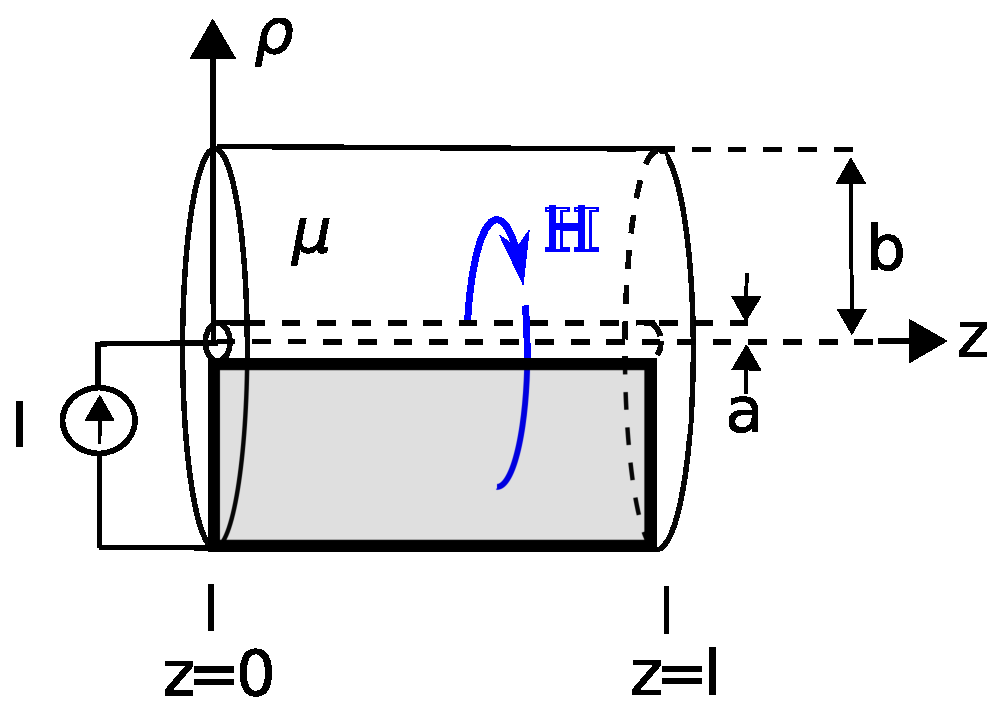
\includegraphics[width=2.5in]{modules/m0125_IndCoax.eps}
}}{Two concentric cylindrical conductors of radii a (inner) and b (outer), centered horizontally over the z-axis with length from z=0 to z=l. The permeability of the region between the cylinders is mu. A vector, rho, extends upward from the center conductor. Current is shown clockwise moving from outer to inner. Between the inner and outer conductor, is a blue 3D circle labeled H coming out of the page. The cross-section is shown as a bold, shaded rectangle. }
\end{center} 
% ***WikipediaCommonsURL
%\centerline{\scriptsize 
%\copyright~\hyperref[m0113_fCapCoax_Credit]{author} 
%\href{https://creativecommons.org/licenses/by-sa/4.0/}{CC BY~SA 4.0} 
%} 
\caption{
\label{m0125_fIndCoax}
Determining the inductance of coaxial line.
}
\end{figure}

Below we shall find the inductance by assuming a current $I$ on the inner conductor and integrating over the resulting magnetic field to obtain the magnetic flux $\Phi$ between the conductors.  Then, inductance can be determined as the ratio of the response flux to the source current.

Before we get started, note the derivation we are about to do is similar to the derivation of the \emph{capacitance} of a coaxial structure, addressed in Section~\ref{m0113_Capacitance_of_Coaxial_Line}.  The reader may benefit from a review of that section before attempting this derivation.

The first step is to find the magnetic field inside the structure.
This is relatively simple if we may neglect fringing fields, 
\index{fringing (field)}
since then the internal field may be assumed to be constant with respect to $z$.
This analysis will also apply to the case where the length $l$ pertains to one short section of a much longer structure; in this case we will obtain the inductance \emph{per length} as opposed to the total inductance for the structure.
Note that the latter is exactly what we need for the transmission line lumped-element equivalent circuit model (Section~\ref{m0029_Lumped-Element_Model}).

To determine the inductance, we invoke the definition (Section~\ref{m0123_Inductance}):
%
\begin{equation}
L \triangleq \frac{\Phi}{I}
\label{m0125_eIndDef}
\end{equation}
%
A current $I$ flowing in the $+z$ direction on the inner conductor gives rise to a magnetic field inside the coaxial structure.
The magnetic field intensity for this scenario was determined in Section~\ref{m0119_Magnetic_Field_of_a_Long_Wire} where we found
%
\begin{equation}
{\bf H} = \hat{\phi} \frac{I}{2\pi \rho} ~~, ~~ a \le\rho\le b
\end{equation}
%
The reader should note that in that section we were considering merely a line of current; not a coaxial structure.
So, on what basis do we claim the field for inside the coaxial structure is the same?
This is a consequence of Ampere's Law 
\index{Ampere's law!magnetostatics}
(Section~\ref{m0019_Amperes_Law_Magnetostatics}):
%
\begin{equation}
\oint_{\mathcal C} {\bf H}\cdot d{\bf l} = I_{encl}
\end{equation}
%
If in this new problem we specify the same circular path $\mathcal{C}$ with radius greater than $a$ and less than $b$, then the enclosed current is simply $I$.
The presence of the outer conductor does not change the radial symmetry of the problem, and nothing else remains that can change the outcome.
This is worth noting for future reference:
%
%ORB HIGHLIGHT
\begin{mdframed}[backgroundcolor=yellow!20,nobreak=true] 
The magnetic field inside a coaxial structure comprised of concentric conductors bearing current $I$ is identical to the magnetic field of the line current $I$ in free space.
\end{mdframed}

We're going to need magnetic flux density (${\bf B}$) as opposed to ${\bf H}$ in order to get the magnetic flux.
This is simple since they are related by the permeability of the medium; i.e., ${\bf B}=\mu{\bf H}$.
Thus:
%
\begin{equation}
{\bf B} = \hat{\phi} \frac{\mu I}{2\pi \rho} ~~, ~~ a \le\rho\le b
\end{equation}

Next, we get $\Phi$ by integrating over the magnetic flux density
%
\begin{equation}
\Phi = \int_{\mathcal S}{ {\bf B} \cdot d{\bf s} }
\end{equation}
%
where $\mathcal{S}$ is any open surface through which all magnetic field lines within the structure must pass.
Since this can be \emph{any} such surface, we may as well choose the simplest one.
The simplest such surface is a plane of constant $\phi$, since such a plane is a constant-coordinate surface and perpendicular to the magnetic field lines.
This surface is shown as the shaded area in Figure~\ref{m0125_fIndCoax}.
Using this surface we find:
%
\begin{flalign}
\Phi &= \int_{\rho=a}^b \int_{z=0}^l { \left( \hat{\bf \phi} \frac{\mu I}{2\pi\rho} \right) \cdot \left(\hat{\bf \phi}~d\rho~dz\right) }  \nonumber \\
%  &=  \frac{\mu I}{2\pi} \int_{\rho=a}^b \int_{z=0}^l { \frac{d\rho}{\rho} dz }  \nonumber \\
  &=  \frac{\mu I}{2\pi} \left( \int_{z=0}^l { dz } \right)  \left( \int_{\rho=a}^b { \frac{d\rho}{\rho} } \right)  \nonumber \\
  &=  \frac{\mu I l}{2\pi} \ln\left(\frac{b}{a}\right)
\end{flalign} 

Wrapping up:
%
\begin{equation}
L \triangleq \frac{\Phi}{I} = \frac{\left(\mu Il/2\pi\right)\ln\left(b/a\right) }{ I }
\end{equation}
% 
Note that factors of $I$ in the numerator and denominator cancel out, leaving:
%
\begin{equation}
\boxed{
L = \frac{\mu l}{2\pi} \ln\left(\frac{b}{a}\right)   
}
\end{equation}
%
Note that this is dimensionally correct, having units of H. 
Also note that this is expression depends only on materials (through $\mu$) and geometry (through $l$, $a$, and $b$).
Notably, it does \emph{not} depend on current, which would imply non-linear behavior.

To make the connection back to lumped-element transmission line model parameters (Sections~\ref{m0029_Lumped-Element_Model} and \ref{m0143_Coaxial_Line}), we simply divide by $l$ to get the per-unit length parameter:
%
\begin{equation}
\boxed{
L' = \frac{\mu}{2\pi} \ln\left(\frac{b}{a}\right)   
}
\label{m0125_eLp}
\end{equation}
%
which has the expected units of H/m.

%--------------------------------

%ORB EXAMPLE
~\\ \begin{example} 
\begin{mdframed}[backgroundcolor=brown!20,linecolor=brown!20]\raggedright
Inductance of RG-59 coaxial cable.
\\~\\
RG-59 coaxial cable consists of an inner conductor having radius $0.292$~mm, an outer conductor having radius $1.855$~mm, and polyethylene (a non-magnetic dielectric) spacing material.
Estimate the inductance per length of RG-59.

{\bf Solution.}  From the problem statement, 
$a=0.292$~mm, 
$b=1.855$~mm, 
and $\mu \cong \mu_0$ since the spacing material is non-magnetic.
Using Equation~\ref{m0125_eLp}, we find $L'\cong 370$~nH/m.
\end{mdframed}\end{example}

\index{inductor!coaxial|)}
